% To je predloga za poročila o domačih nalogah pri predmetih, katerih
% nosilec je Blaž Zupan. Seveda lahko tudi dodaš kakšen nov, zanimiv
% in uporaben element, ki ga v tej predlogi (še) ni. Več o LaTeX-u izveš na
% spletu, na primer na http://tobi.oetiker.ch/lshort/lshort.pdf.
%
% To predlogo lahko spremeniš v PDF dokument s pomočjo programa
% pdflatex, ki je del standardne instalacije LaTeX programov.

\documentclass[a4paper,11pt]{article}
\usepackage{a4wide}
\usepackage{fullpage}
\usepackage[utf8x]{inputenc}
\usepackage[slovene]{babel}
\selectlanguage{slovene}
\usepackage[toc,page]{appendix}
\usepackage[pdftex]{graphicx} % za slike
\usepackage{setspace}
\usepackage{color}
\definecolor{light-gray}{gray}{0.95}
\usepackage{listings} % za vključevanje kode
\usepackage{hyperref}
\usepackage{float}
\usepackage{verbatim}
\renewcommand{\baselinestretch}{1.2} % za boljšo berljivost večji razmak
\renewcommand{\appendixpagename}{Priloge}

\lstset{ % nastavitve za izpis kode, sem lahko tudi kaj dodaš/spremeniš
language=Python,
basicstyle=\footnotesize,
basicstyle=\ttfamily\footnotesize\setstretch{1},
backgroundcolor=\color{light-gray},
}

\title{Šesta domača naloga}
\author{Anže Pečar (63060257)}
\date{\today}

\begin{document}

\maketitle

\section{Uvod}
Namen "seste doma"ce naloge je seznaniti se z podatki za tekmovanje iz podro"cja kemoinformatike. 

\section{Podatki in opis problemske domene}

\section{Informativnost atributov}
\section{Ocenjevanje kakovosti napovednih modelov}
%\begin{figure}[H]
%\begin{center}
%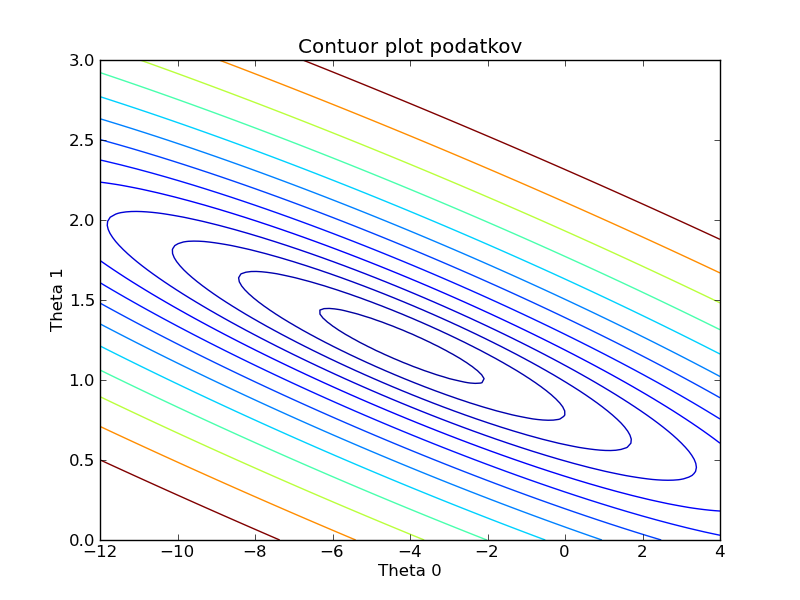
\includegraphics[scale=0.3]{contour.png}
%\caption{Prikaz J funkcije}
%\end{center}
%\label{contour}
%\end{figure}



\section{Izjava o izdelavi domače naloge}
Domačo nalogo in pripadajoče programe sem izdelal sam.


\begin{thebibliography}{9}

\bibitem{mining}
   Ian H. Witten \& Eibe Frank,
   \emph{Data Mining Practical Machine Learning Tools and Techniques, Second Edition}
   Morgan Kaufmann Publishers,  
   2005.

\end{thebibliography}

\end{document}
